\chapter{\ifproject%
\ifenglish Project Structure and Methodology\else โครงสร้างและขั้นตอนการทำงาน\fi
\else%
\ifenglish Project Structure\else โครงสร้างของโครงงาน\fi
\fi
}
\makeatletter

% \renewcommand\section{\@startsection {section}{1}{\z@}%
%                                    {13.5ex \@plus -1ex \@minus -.2ex}%
%                                    {2.3ex \@plus.2ex}%
%                                    {\normalfont\large\bfseries}}

\makeatother
%\vspace{2ex}
% \titleformat{\section}{\normalfont\bfseries}{\thesection}{1em}{}
% \titlespacing*{\section}{0pt}{10ex}{0pt}
\hspace{\parindent} ในบทนี้จะกล่าวถึงโครงสร้างภาพรวม และหลักการออกแบบของระบบบริหารจัดการพลังงานอัจฉริยะ
เพื่อมุ่งสู่ความเป็นกลางทางคาร์บอนในอาคาร โดยระบบบ่งออกเป็น 3 ส่วนหลัก คือ สถานีวัดสภาพอากาศขนาดย่อม, 
โมเดลการทำนายการผลิตไฟฟ้าจากโซลาร์เซลล์ล่วงหน้า 24 ชั่วโมง และเซิฟเวอร์และเว็บไซต์สำหรับแสดงผล

\begin{figure}[H]
    \centering
    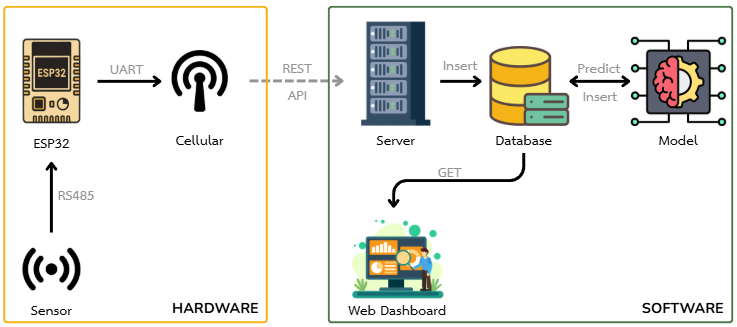
\includegraphics[width=0.7\textwidth]{images/chapter_3/overview.png} 
    \caption{แผนภาพแสดงการทำงานของระบบ}
    \label{fig:overview daigram}
\end{figure}

\section{สถานีวัดสภาพอากาศขนาดย่อม}
\subsection{โครงสร้างสถานีวัดสภาพอากาศขนาดย่อม}
\hspace{\parindent} โครงสร้างของสถานีวัดสภาพอากาศขนาดย่อมแบ่งเป็น 3 ส่วนหลัก คือ ระบบจ่ายไฟฟ้า, ชุดควบคุมหลัก และเซนเซอร์ตรวจวัดสภาพแวดล้อม 
โดยการเชื่อมต่อระหว่างชุดควบคุมหลักและเซนเซอร์ตรวจวัดสภาพแวดล้อมใช้การสื่อสารแบบ RS485 โดยการออกแบบจะเน้นไปที่การป้องกัน SPOF 
(Single Point of Failure), ซ่อมแซมง่าย, ประหยัดพลังงาน และเพิ่มความน่าเชื่อถือให้ระบบ
% Fix
\begin{figure}[H]
    \centering
    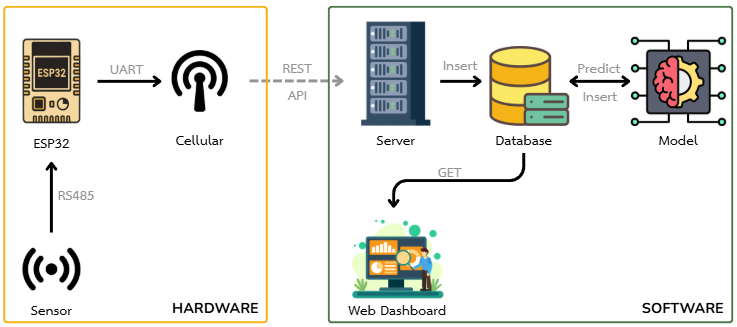
\includegraphics[width=0.7\textwidth]{images/chapter_3/overview.png} 
    \caption{แผนภาพแสดงการทำงานของระบบ}
    \label{fig:overview daigram}
\end{figure}

\subsection{อุปกรณ์ที่ใช้ในสถานีวัดสภาพอากาศขนาดย่อม}
\textbf{ระบบจ่ายไฟฟ้า} \\

\hspace{\parindent} ระบบใช้ไฟฟ้ากระแสตรงขนาด 12 โวลต์จากแหล่งจ่ายภายนอก และทำการแปลงแรงดันไฟฟ้าให้เหมาะสมกับอุปกรณ์แต่ละชนิด เช่น 5 โวลต์สำหรับไมโครคอนโทรลเลอร์ 
และ 3.3 โวลต์สำหรับเซนเซอร์บางประเภทโดยใช้โมดูล LM2596 และแหล่งจ่ายพลังงานสามารถปรับเปลี่ยนได้ตามสภาพแวดล้อมการติดตั้ง เช่น การใช้ระบบโซลาร์เซลล์หรืออะแดปเตอร์ไฟฟ้า 
ทั้งนี้การออกแบบระบบจ่ายไฟคำนึงถึงความเสถียรและการประหยัดพลังงานเป็นหลัก

\textbf{ชุดควบคุมหลัก}
% Fix
\begin{table}[h]
\centering
\begin{tabular}{|l|l|l|}
\hline
\textbf{อุปกรณ์} & \textbf{หน้าที่} & \textbf{การเชื่อมต่อ} \\ \hline
ESP32 & หน่วยควบคุมหลัก & - \\ \hline
SIMA7670E & ส่งข้อมูลไปที่ Server & UART \\ \hline
MAX485 & สื่อสารกับเซนเซอร์ผ่าน RS485 & RS485 \\ \hline
Relay Module & ควบคุมการจ่ายไฟฟ้าให้เซนเซอร์ & Digital (HIGH/LOW) \\ \hline
\end{tabular}
\caption{ตารางแสดงอุปกรณ์หลักในชุดควบคุมและการเชื่อมต่อ}
\label{tab:main control}
\end{table}

\hspace{\parindent} การเลือกใช้ RS485 ช่วยให้ระบบสามารถสื่อสารในระยะไกลและทนต่อสัญญาณรบกวนได้ดี เหมาะสำหรับการติดตั้งภายนอกอาคาร \\

\textbf{เซนเซอร์ตรวจวัดสภาพแวดล้อม}

\begin{table}[h]
\centering
\begin{tabular}{|l|l|c|l|}
\hline
\textbf{เซนเซอร์} & \textbf{หน้าที่} & \textbf{การเชื่อมต่อ} & \textbf{ความละเอียด} \\ \hline
\multirow{3}{*}{BME280} & วัดอุณหภูมิ & \multirow{3}{*}{I2C} & 0.01 $^\circ$C \\ \cline{2-2} \cline{4-4} 
 & วัดความชื้น &  & 0.008\% \\ \cline{2-2} \cline{4-4} 
 & วัดความกดอากาศ &  & 1 hPa \\ \hline
VEML7700 & วัดความเข้มแสง & I2C & 0.0036 Lux/CT \\ \hline
Wind Speed Sensor & วัดความเร็วลม & RS485 & 0.1 m/s \\ \hline
Wind Direction Sensor & วัดทิศทางลม & RS485 & 1$^\circ$ \\ \hline
PT100 & วัดอุณหภูมิ ณ จุดสัมผัส & RTD & 0.1 $^\circ$C \\ \hline
\end{tabular}
\caption{ตารางแสดงอุปกรณ์เซนเซอร์ที่ใช้ในสถานีวัดสภาพอากาศขนาดย่อม}
\label{tab:sensor list}
\end{table}

\hspace{\parindent} เซนเซอร์ที่ใช้การสื่อสารแบบ I2C และ RTD จะถูกแปลงสัญญาณเป็น RS485 เพื่อให้สามารถรวมอยู่ในระบบสื่อสารเดียวกัน ลดความซับซ้อนของระบบและเพิ่มความสามารถในการขยายในอนาคต \\

% Fix
\begin{figure}[H]
    \centering
    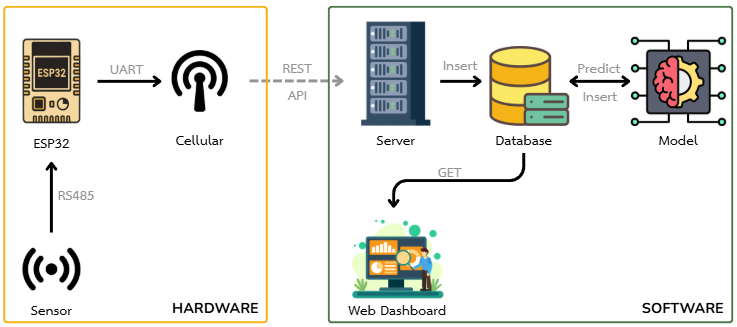
\includegraphics[width=0.7\textwidth]{images/chapter_3/overview.png} 
    \caption{แผนภาพแสดงการทำงานของระบบ}
    \label{fig:overview daigram}
\end{figure}

\begin{itemize}
    \item [] \textbf{3.1.2.1 การแปลงสัญญาณจาก I2C เป็น RS485 (I2C to RS485 Conversion)} \\ 
    \hspace{\parindent} จากตารางที่ \ref{tab:sensor list} จะเห็นว่าเซนเซอร์จำนวน 2 ตัว ได้แก่ BME280 และ VEML7700 ใช้การสื่อสารแบบ I2C ซึ่งเหมาะสำหรับการสื่อสารระยะสั้นภายในบอร์ดเดียวกัน 
    อย่างไรก็ตาม I2C มีข้อจำกัดด้านระยะทางและความทนทานต่อสัญญาณรบกวน จึงไม่เหมาะสมสำหรับการใช้งานในระบบที่ต้องติดตั้งเซนเซอร์ในระยะไกล
    \item [] \textbf{3.1.2.2 การแปลงสัญญาณจาก RTD เป็น RS485 (RTD to RS485 Conversion)} \\ 
    \hspace{\parindent} จากตารางที่ \ref{tab:sensor list} จะเห็นว่าเซนเซอร์ PT100 ที่ใช้ในการวัดอุณหภูมิ ณ บริเวณแผงโซลาร์เซลล์ ซึ่งเป็นเซนเซอร์ที่ทำงานโดยอาศัยการเปลี่ยนแปลงค่าความต้านทานตามอุณหภูมิ ซึ่งไม่สามารถเชื่อมต่อเข้ากับไมโครคอนโทรลเลอร์โดยตรงได้ จำเป็นต้องมีวงจรแปลงสัญญาณเพื่อแปลงค่าความต้านทานให้อยู่ในรูปแบบสัญญาณไฟฟ้าที่สามารถประมวลผลได้ \\
    
    \hspace{\parindent} ในการออกแบบระบบนี้ ได้มีการใช้โมดูลแปลงสัญญาณ RTD เป็น RS485 ซึ่งภายในโมดูลจะทำหน้าที่แปลงค่าความต้านทานของ PT100 ให้เป็นข้อมูลดิจิทัล และส่งออกผ่านการสื่อสารแบบ RS485 โดยใช้โปรโตคอล Modbus RTU ทำให้สามารถเชื่อมต่อเข้ากับระบบหลักได้โดยตรง \\
    กระบวนการทำงานของระบบสามารถอธิบายได้ดังนี้
    
    \begin{enumerate}
        \item โมดูล RTD ทำการวัดค่าความต้านทานจากเซนเซอร์ PT100
        \item แปลงค่าความต้านทานเป็นค่าอุณหภูมิด้วยวงจรภายใน
        \item จัดเก็บข้อมูลในรูปแบบรีจิสเตอร์ของ Modbus
        \item ส่งข้อมูลผ่าน RS485 เมื่อได้รับคำสั่งจากอุปกรณ์ Master
    \end{enumerate}
    
    \hspace{\parindent} การออกแบบลักษณะนี้ช่วยลดภาระการประมวลผลของไมโครคอนโทรลเลอร์ เนื่องจากการแปลงค่าทางกายภาพเป็นข้อมูลดิจิทัลถูกจัดการภายในโมดูลแล้ว อีกทั้งยังช่วยเพิ่มความแม่นยำของข้อมูล และลดความซับซ้อนในการออกแบบวงจร
    นอกจากนี้ การใช้การสื่อสารแบบ RS485 ยังช่วยให้สามารถติดตั้งเซนเซอร์ในระยะไกลได้ และมีความทนทานต่อสัญญาณรบกวน เหมาะสำหรับการใช้งานในสภาพแวดล้อมจริง

    \item [] \textbf{3.1.2.3 การสื่อสารข้อมูลด้วย RS485 และ Modbus RTU (RS485 and Modbus RTU Communication)} \\ 
    \hspace{\parindent} ภายในระบบสถานีวัดสภาพอากาศขนาดย่อม ได้เลือกใช้การสื่อสารแบบ RS485 ร่วมกับโปรโตคอล Modbus RTU เป็นกลไกหลักในการรับส่งข้อมูลระหว่างอุปกรณ์ต่าง ๆ เนื่องจาก RS485 มีความสามารถในการสื่อสารในระยะไกล และมีความทนทานต่อสัญญาณรบกวน เหมาะสำหรับการติดตั้งในสภาพแวดล้อมภายนอกอาคาร
    
    \hspace{\parindent} ในระบบนี้ โครงสร้างการสื่อสารออกแบบมาในลักษณะ Master-Slave โดยมีชุดควบคุมหลักทำหน้าที่เป็น Master และอุปกรณ์เซนเซอร์ทำหน้าที่เป็น Slave ซึ่งแต่ละอุปกรณ์จะมีหมายเลขประจำตัว (Slave ID) ดังนี้
    \begin{table}[h]
    \centering
    \begin{tabular}{|l|l|}
    \hline
    \textbf{อุปกรณ์} & \textbf{SlaveID} \\ \hline
    Wind Speed Sensor & 1 \\ \hline
    Wind Direction Sensor & 2 \\ \hline
    PT100 & 3 \\ \hline
    Sensor Node & 4 \\ \hline
    \end{tabular}
    \end{table}

    กระบวนการสื่อสารสามารถอธิบายได้ดังนี้
    \begin{enumerate}
        \item อุปกรณ์ Master ส่งคำสั่ง (Request) ไปยัง Slave ตามหมายเลข Slave ID
        \item Slave ที่ถูกเรียกจะตอบกลับข้อมูล (Response) ตามคำสั่งที่ได้รับ
        \item ข้อมูลจะถูกส่งในรูปแบบของเฟรมข้อมูลตามมาตรฐาน Modbus RTU
        \item Master ทำการรวบรวมข้อมูลจาก Slave หลายตัวเพื่อส่งไปยัง Server
    \end{enumerate}

    \hspace{\parindent} การออกแบบในลักษณะนี้ช่วยให้สามารถเชื่อมต่ออุปกรณ์หลายตัวบนสายสื่อสารเดียวกัน ลดจำนวนสายสัญญาณ และเพิ่มความสามารถในการขยายระบบในอนาคต \\
    \hspace{\parindent} นอกจากนี้ การใช้ Modbus RTU ซึ่งเป็นโปรโตคอลมาตรฐาน ยังช่วยให้สามารถรองรับอุปกรณ์จากผู้ผลิตที่หลากหลาย และเพิ่มความยืดหยุ่นในการพัฒนาระบบ

\end{itemize}

\subsection{หลักการทำงานของสถานีวัดสภาพอากาศขนาดย่อม}

\hspace{\parindent} สถานีวัดสภาพอากาศขนาดย่อมถูกออกแบบให้ทำงานในลักษณะของระบบกระจาย (Distributed System) โดยมีการสื่อสารระหว่างอุปกรณ์ผ่านเครือข่าย RS485 
และใช้โปรโตคอล Modbus RTU ในการรับส่งข้อมูล เพื่อรองรับการติดตั้งเซนเซอร์ในระยะไกลและเพิ่มความทนทานต่อสัญญาณรบกวน \\
% ใส่รูป
\hspace{\parindent} การทำงานของระบบสามารถแบ่งออกเป็น 3 ช่วงหลัก ได้แก่ การเริ่มต้นระบบ การตรวจสอบอุปกรณ์ และการเก็บข้อมูล โดยมีลำดับการทำงานดังนี้

\begin{enumerate}
    \item ขั้นตอนการเริ่มต้นระบบ (Initialization Phase)
    \begin{enumerate}
        \item ระบบจ่ายไฟให้กับชุดควบคุมหลัก
        \item ชุดควบคุมหลักทำการกำหนดค่าเริ่มต้นและตรวจสอบการเชื่อมต่อของอุปกรณ์ (Hardware Initialization)
    \end{enumerate}

    \item ขั้นตอนการตรวจสอบอุปกรณ์ (Device Checking Phase)
    \begin{enumerate}
        \item ชุดควบคุมหลักส่งคำสั่งไปยังอุปกรณ์แต่ละตัวเพื่อตรวจสอบสถานะการทำงาน
        \item อุปกรณ์ตอบกลับสถานะผ่านโปรโตคอล Modbus RTU
        \item ระบบส่งข้อมูลสถานะการทำงานของอุปกรณ์ไปยัง Server
        \item ระบบเข้าสู่โหมดประหยัดพลังงาน (Deep Sleep) เป็นระยะเวลา 15 นาที
        \item ทำซ้ำขั้นตอนที่ 3–6 เป็นจำนวน 4 รอบ เพื่อยืนยันความพร้อมของระบบก่อนเริ่มการเก็บข้อมูลจริง
    \end{enumerate}

    \item ขั้นตอนการเก็บและส่งข้อมูล (Data Acquisition Phase)
    \begin{enumerate}
        \item ชุดควบคุมหลักร้องขอข้อมูลจากเซนเซอร์ทั้งหมดผ่าน RS485
        \item เซนเซอร์ส่งค่าที่ตรวจวัดได้กลับมาในรูปแบบ Modbus Register
        \item ระบบทำการรวบรวมและจัดรูปแบบข้อมูล
        \item ส่งข้อมูลไปยัง Server ผ่านโมดูลสื่อสาร
        \item ระบบเข้าสู่โหมด Deep Sleep และวนกลับไปทำงานในขั้นตอนที่ 8
    \end{enumerate}
\end{enumerate}

\hspace{\parindent} การออกแบบลักษณะนี้ช่วยให้ระบบสามารถตรวจสอบความพร้อมของอุปกรณ์ก่อนเริ่มการทำงานจริง ลดความผิดพลาดในการเก็บข้อมูล และช่วยประหยัดพลังงานผ่านการใช้โหมด Deep Sleep อีกทั้งยังเพิ่มความน่าเชื่อถือของระบบโดยรวม

\section{โมเดลการทำนายการผลิตไฟฟ้าจากโซลาร์เซลล์}
\subsection{ภาพรวมของโมเดล (Model Overview)}
\subsection{ขั้นตอนการพัฒนาโมเดล (Model Development Process)}

\section{เซิฟเวอร์และเว็บไซต์สำหรับแสดงผล}
\subsection{ภาพรวมของระบบ (System Overview)}
\subsection{เทคโนโลยีและเครื่องมือที่ใช้ (Technology Stack and Tools)}
\subsection{การออกแบบฐานข้อมูลและการจัดการข้อมูล (Database Design and Data Management)}
\subsection{การออกแบบ API(Application Programming Interface)}
\subsection{การออกแบบส่วนติดต่อผู้ใช้และเว็บไซต์ (Frontend and User Interface Design)}